\documentclass[a4,landscape]{seminar}
\usepackage[utf8x]{inputenc}
\usepackage[pdftex]{graphicx}
\usepackage{fancybox}
\usepackage{url}
% \usepackage{sem-a4}

\pdfcompresslevel=9
\pdfpageheight=8.27truein
\pdfpagewidth=11.69truein
\pdfhorigin=1truein
\pdfvorigin=1truein
\slideheight 14truein
\slidewidth 22truein

\newpagestyle{roberts}
        {\thepage\hfil Introduction to Emacs and TextMate 2017\hfil\hfil\hfil\hfil\hfil\hfil Fei Roth \texttt{fei.roth@gu.se}\hfil}{}
\pagestyle{roberts}
\slideframe{oval}

\begin{document}
\begin{slide}
  {\Large Emacs}\\[1ex]
  Emacs is a text editor from the mid 70's by Richard Stallman. Ported to Mac, Windows, Linux\dots and works basically the same way on all systems. Though, derivatives may have custom behavior, eg Aquamacs for Mac, or EmacsW32 for Windows. Emacs is open free software.
\begin{itemize}
  \item Starting Emacs (or Aquamacs)\\[1ex]
    Start Emacs either by
    \begin{itemize}
    \item typing the command \texttt{emacs} on a command-line,
    \item typing \texttt{emacs ARG} where \texttt{ARG} is a path to a file to be opened, or
    \item starting it from Finder under the Applications folder.
    \end{itemize}
    After starting a startup screen with various information will be
    displayed, pressing \texttt{q} in this window will get rid of it.
    \clearpage{}
  \item The Emacs Window\\[1ex]
    In addition to the usual toolbar at the top of the Emacs window, notice
    \begin{enumerate}
    \item the \emph{buffer} where you can write texts/programs etc,
    \item the \emph{statusbar} shows condensed info about the buffer immediately above it, and
    \item the \emph{minibuffer} which Emacs uses to request information. Even when using the menubar or toolbar buttons it can ask for input in the minibuffer. The\\keyboard shortcut \texttt{C-g} will quit any interaction in the minibuffer.
    \end{enumerate}\vspace{5mm}
    \begin{center}
      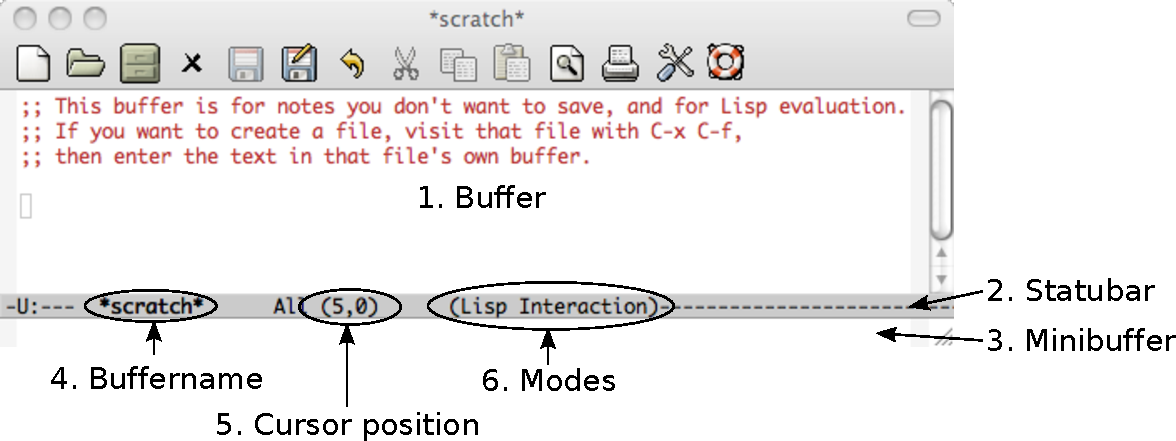
\includegraphics[scale=.55]{emacs-image.pdf}
    \end{center}
    \clearpage{}
    In the statusbar
    \begin{enumerate}
      \setcounter{enumi}{3}
    \item the buffer's name, often filename, will be displayed,
    \item the position of the caret \texttt{(row,col)}, and
    \item what mode is currently used.
    \end{enumerate}
    The statusbar also shows if the buffer is saved etc.
  \item Modes\\[1ex]
    A mode adapts the editor's behaviour. It can be set automatically
    when opening a file depending on the file type. Emacs can also be forced
    to change mode by typing a command in the minibuffer, eg\\[1ex]
    \texttt{M-x python-mode}\\[1ex]
    will change the current buffer's mode so Emacs will assist in
    python programming. \clearpage{}
  \item Commands, \texttt{M-x}\\[1ex]
    Emacs can also, apart from the menu- and toolbar, be controlled by
    issuing commands in the minibuffer.  Press the keyboard shortcut
    \texttt{M-x} followed by a \texttt{COMMAND}. \texttt{M-} is the
    \texttt{<alt>}-key on our Macs, and corresponds eg to the
    \texttt{esc}-key on other systems.\\[1ex]
    N.B. The ordinary Mac \texttt{<cmd>-X} shortcuts etc do not work
    when running Emacs on our Macs.\\[1ex]
    Two really important commands\\[1ex]
    \texttt{M-x doctor} and  \texttt{M-x tetris}\\[1ex]
    Jokes aside, using Emacs one will some day need to issue commands
    using \texttt{M-x COMMAND}.\\[1ex]
    The minibuffer can be \texttt{<TAB>}-completed\dots eg\\[1ex]
    \texttt{M-x <TAB><TAB><TAB>\dots}
    \clearpage{}
  \item Keyboard Shortcuts \\\\
    Emacs is known for its numerous keyboard shortcuts. \\
    Please review some examples for common shortcuts in the attached
    PDF documents.\\[1ex]
    Again, the ordinary Mac \texttt{<cmd>-X} shortcuts etc do not
    work. Remember \texttt{M-} is the \texttt{<alt>}-key and
    \texttt{C-} is the \texttt{<ctrl>}-key.\\[1ex]
    N.B. Some keyboard shortcuts will ask for input in the minibuffer, eg \texttt{C-x C-f} will ask for a filename.
    \clearpage{}
  \item Python Programming in Emacs\\[1ex]
    When writing Python programs, make sure that the mode is set to
    Python, which will give you
    \begin{itemize}
    \item the Python menubar,
    \item syntax highlighting, and
    \item Python indentation etc.
    \end{itemize}
    To run a Python program inside Emacs, type the keyboard shortcut
    \texttt{C-c C-c} and view the buffer \texttt{*Python*} using the
    buffer management shortcuts above.
  \end{itemize}
\end{slide}
\begin{slide}
  {\Large TextMate}\\[1ex]
  TextMate is a text editor like Emacs, but Macified, developed by the
  company Macromates. Works on MacOS X only. Also, TextMate is closed
  proprietory software that comes with a small fee. Though, it's free
  to develop plug-ins/bundles.
\begin{itemize}
  \item Starting TextMate\\[1ex]
    Start TextMate either by
    \begin{itemize}
    \item typing the command \texttt{mate} on a command-line (ln -s
      \url{/Applications/TextMate.app/Contents/Resources/mate} \url{/usr/local/bin/mate}),
    \item typing \texttt{mate ARG} where \texttt{ARG} is a path to a file to be opened, or
    \item starting it from Finder under the Applications folder.
    \end{itemize}
    After starting the program, a startup screen with various information will be
    displayed. You can close this window.
    \clearpage{}
  \item The TextMate Window\\[1ex]
    In addition to the usual menubar at the top and the document area
    where you can write texts/programs, please notice
    \begin{enumerate}
    \item the \emph{mode menu} for changing mode, and 
    \item the \emph{bundle menu} for running misc commands.
    \end{enumerate}\vspace{5mm}
    \begin{center}
      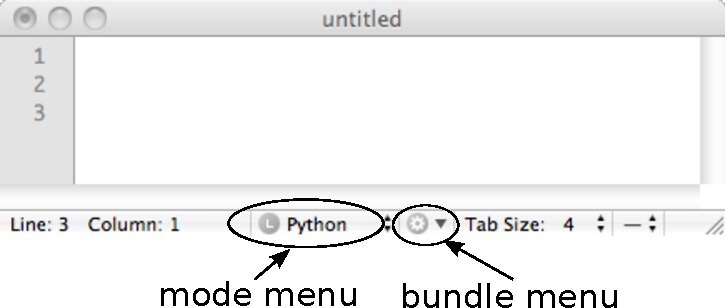
\includegraphics[scale=.7]{drawing.pdf}
    \end{center}
    \clearpage{}
  \item Python Programming in TextMate\\[1ex]
    When writing programs in Python, please make sure that the mode menu is set to
    Python which will give you
    \begin{itemize}
    \item syntax highlightning, and
    \item Python indentation etc.
    \end{itemize}
    To run a Python program inside TextMate, you press the Apple keyboard shortcut
    \texttt{<cmd>-R}.
  \end{itemize}
\end{slide}
\begin{slide}
  {\Large Refs}\\[1ex]
    \url{http://www.gnu.org/software/emacs/}\\
    \url{http://en.wikipedia.org/wiki/Emacs}\\
    \url{http://manual.macromates.com/en/}
\end{slide}
\end{document}